%%%%%%%%%%%%%%%%%%%%%%%%%%%%%%%%%%%%%%%%%
% Presentation Template
% LaTeX Template
% Version 2.0 (2023-06-16)
%
% This template was adapted by:
% Jonathan Decker (jonathan.decker@uni-goettingen.de)
% From a template made by:
% Julian Kunkel (julian.kunkel@gwdg.de)
%
%%%%%%%%%%%%%%%%%%%%%%%%%%%%%%%%%%%%%%%%%
\documentclass[compress,aspectratio=169]{beamer}

% make sure the theme and config files are on this path
% uncomment the required theme setting
\usepackage[HPS]{assets/beamerConfig}
%\usepackage[GWDG]{assets/beamerConfig}
%\usepackage[DECICE]{assets/beamerConfig}

\addbibresource{ref.bib}
\graphicspath{{.}{assets/}}

% --- document configuration ---
\newcommand{\mytitle}{MPI-based Creation and Benchmarking of\\a Dynamic Elasticsearch Cluster}
% Leave empty for no subtitle
\newcommand{\mysubtitle}{}
\newcommand{\myauthor}{Lars Quentin}
\newcommand{\myauthorurl}{https://hpc.gwdg.de}
\newcommand{\myvenue}{SCAP}
% For example, use \today
\newcommand{\mydate}{11.07.2024}
% For example, Institute for Computer Science / GWDG
\newcommand{\myinstitute}{University of G\"ottingen}

\newcommand{\ccheckmark}{\mbox{\ooalign{$\checkmark$\cr\hidewidth$\square$\hidewidth\cr}}}
\newcommand{\ccheckbox}{\mbox{$\square$}}

\configuretitlepage

\begin{document}
	\begin{frame}[plain]
		\titlepage
	\end{frame}

	\begin{frame}[t]{}
		\tableofcontents[subsectionstyle=hide/hide]
	\end{frame}

	% --- slides begin ---

	\section{Introduction}
	\begin{frame}{Insights}
		\begin{itemize}
			\item Why a custom spawner and new specialized benchmarker is required
      \item How the following works:
        \begin{itemize}
          \item distributed cluster spawner
          \item distributed ingestion benchmarker
          \item distributed query benchmarker
        \end{itemize}
      \item How to create a new benchmark scenario from scratch
		\end{itemize}
	\end{frame}

  \begin{frame}{Motivation: Data Lakes}
    \begin{columns}
      \begin{column}{0.5\textwidth}
        \begin{block}{Why are Data Lakes needed}
          \begin{itemize}
            \item Research becomes evermore data-driven and compute-intensive
              \begin{itemize}
                \item More Simulations
                \item Data Science, Machine Learning
              \end{itemize}
            \item HPC becomes more data oriented
            \item Better data-management tooling needed
            \item HPC operates on raw data\\$\Rightarrow$ Data Lakes
          \end{itemize}
        \end{block}
      \end{column}
      \pause
      \begin{column}{0.5\textwidth}
        \begin{block}{Metadata management}
          \begin{itemize}
            \item Providing storage is easy
            \item Managing storage is hard
            \item Keep data findable, manage data
            \item Fully indexed
            \item Fully (fuzzy) searchable
            \item No-SQL data store / search engine
              \begin{itemize}
                \item Elasticsearch
              \end{itemize}
          \end{itemize}
        \end{block}
      \end{column}
    \end{columns}
  \end{frame}

  \begin{frame}{Motivation: Elasticsearch and Rally}
    \begin{columns}
      \begin{column}{0.5\textwidth}
        \begin{block}{Elasticsearch for HPC}
          \begin{itemize}
            \item Elasticsearch is designed for cloud-use
              \begin{itemize}
                \item Always running
                \item Same host, same IP
                \item Only ethernet
              \end{itemize}
            \item This is not given in HPC:
              \begin{itemize}
                \item Jobs spawned on demand
                \item Every job gets different nodes
                \item Changing IPs between runs
                \item ETH, IB, Intel OPA
              \end{itemize}
            \item Thus, a custom \textbf{stateful} workflow is required for HPC use!
          \end{itemize}
        \end{block}
      \end{column}
      \pause
      \begin{column}{0.5\textwidth}
        \begin{block}{Benchmarking Elasticsearch}
          \begin{itemize}
            \item HPC is all about performance
            \item Elastic's benchmarker: \emph{rally} \cite{es_benchmarking}
              \begin{itemize}
                \item Used for in-house performance regression testing
                \item Written in Python
                \item Distributed using \emph{thespian} agent framework
                \item After previous unpublished research at GWDG: 
                  \begin{itemize}
                    \item Doesn't work with over 60 nodes
                  \end{itemize}
              \end{itemize}
              \item Not viable for HPC-scale benchmarking
          \end{itemize}
        \end{block}
      \end{column}
    \end{columns}
  \end{frame}
  
  \begin{frame}{Contributions}
    The 4 main contributions of this work:
    \pause
    \begin{enumerate}
      \item \textbf{On-demand Elasticsearch Cluster Spawner}
        \begin{itemize}
          \item Zero-configuration
          \item Dynamic resolution, based on SLURM MPI envionment
          \item Arbitrary cluster size
          \item Stateful between runs
        \end{itemize}
        \pause
      \item \textbf{Ingestion Benchmarker}
        \begin{itemize}
          \item Distributed, MPI-based
          \item Benchmarks easily portable from rally
        \end{itemize}
        \pause
      \item \textbf{Query Benchmarker}
        \begin{itemize}
          \item Distributed, MPI-based
          \item Mixed queries for realistic load
          \item Custom scenario support using own JSON-based DSL
        \end{itemize}
        \pause
      \item \textbf{Example workflow} for canonical dataset
    \end{enumerate}
  \end{frame}


  \begin{frame}{Background: Elasticsearch}
    \begin{columns}
      \begin{column}{0.5\textwidth}
        \begin{itemize}
          \item Distributed search engine
          \item Document-based NoSQL-Storage
          \item Internally based on Apache Lucene
          \item Provides JSON-based REST interface
          \item Apache 2.0 fork: Opensearch
          \item Advantages:
            \begin{itemize}
              \item Mature ecosystem
              \item Very battle-tested
              \item A lot of tooling / library support
            \end{itemize}
        \end{itemize}
      \end{column}
      \begin{column}{0.5\textwidth}
        \begin{figure}
        
\includegraphics[width=0.8\textwidth]{./assets/es.png}
      \end{figure}
      \end{column}
    \end{columns}
  \end{frame}

  \begin{frame}{Background: Benchmarking}
    \begin{itemize}
      \item For elasticsearch: All literature uses rally \cite{rallyusecase1} \cite{rallyusecase2} \cite{rallyusecase3}
      \item Alternatives: Just use a HTTP benchmarker
        \begin{itemize}
          \item JMeter \cite{jmeter}
          \item wrk \cite{wrk}
          \item Grafana k6 \cite{k6}
        \end{itemize}
      \item Most NoSQL comparisons are done by database vendors \cite{tsbs}
        \begin{itemize}
          \item Bad financial incentives
        \end{itemize}
    \end{itemize}
  \end{frame}

	\section{Spawner}
  \begin{frame}{Contributions}
    \begin{center}
      \begin{itemize}
        \item[\ccheckbox] On-demand Elasticsearch Cluster Spawner
        \item[\ccheckbox] Ingestion Benchmarker
        \item[\ccheckbox] Query Benchmarker
        \item[\ccheckbox] Example workflow for canonical dataset
      \end{itemize}
    \end{center}
  \end{frame}


	\begin{frame}{On-Demand, Dynamic Cluster Spawner}
    \begin{block}{Features}
      \pause
      \begin{itemize}
        \item Fully automated, uses MPI envionment provided by SLURM
          \pause
        \item Dynamically fetches the hosts
          \begin{itemize}
            \item Not required to know them beforehand
            \item IPs and hardware can be changed between runs
          \end{itemize}
          \pause
        \item Very portable through containerization (Singularity)
          \pause
        \item Stateful: Same cluster can be respawned 
          \begin{itemize}
            \item on \textbf{different nodes}
            \item \textbf{without reingestion}
          \end{itemize}
          \pause
        \item NIC-agnostic. Tested on:
          \begin{itemize}
            \item Ethernet
            \item Infiniband
          \end{itemize}
      \end{itemize}
    \end{block}
	\end{frame}

  \begin{frame}{On-Demand, Dynamic Cluster Spawner (cont.)}
    \begin{block}{High-Level Workflow: }
      Prerequisites:
      \begin{itemize}
        \item All hosts are known to each other via the MPI environment
        \item All nodes have at least one shared mount
      \end{itemize}
      \pause
      Workflow:
      \begin{enumerate}
        \item Each node creates a config
          \pause
        \item MPI-Gather all hostnames to the root rank
          \pause
        \item The root node updates the configs for all nodes
          \pause
        \item Each rank stats its singularity container with the config bind-mounted in
      \end{enumerate}
    \end{block}
    \pause
    \begin{center}
      See the accompanying report for a more low-level workflow.
    \end{center}
	\end{frame}

  \begin{frame}[fragile]{On-Demand, Dynamic Cluster Spawner (cont.)}
    \begin{tcolorbox}[title=Example Generated Config]
    \footnotesize\inputminted[xleftmargin=1em,linenos]{yaml}{./assets/escfg.yml}
    \end{tcolorbox}
	\end{frame}

	\section{Ingestor}
  \begin{frame}{Contributions}
    \begin{center}
      \begin{itemize}
        \item[\ccheckmark] On-demand Elasticsearch Cluster Spawner
        \item[\ccheckbox] Ingestion Benchmarker
        \item[\ccheckbox] Query Benchmarker
        \item[\ccheckbox] Example workflow for canonical dataset
      \end{itemize}
    \end{center}
  \end{frame}
  
	\begin{frame}{Ingestion Benchmarker}
    \begin{itemize}
      \item Two purposes:
        \begin{enumerate}
          \item Ingest JSON corpus into Elasticsearch cluster for query benchmarks
          \item Measure performance of \textbf{write-performance} and throughput
        \end{enumerate}
      \item Features:
        \begin{itemize}
          \item Distributed, MPI-based
          \item I/O optimized through \emph{offset caching}
          \item Supports statically typed index definitions
          \item Supports Newline Delimited JSON (NDJSON)
            \begin{itemize}
              \item Thus compatible with rally!
            \end{itemize}
          \item Configurable via CLI: bulk size, shards per node
        \end{itemize}
    \end{itemize}
	\end{frame}

  \begin{frame}{Offset Caching}
    \begin{columns}
      \begin{column}{0.5\textwidth}
        \begin{block}{Problem}
          \begin{itemize}
            \item Data has to be parititioned.
              \pause
            \item This should be done fairly, i.e.\\
              For $N$ nodes and $L$ lines, rank $i$ gets\\
               $\left[ \frac{i}{N} \cdot L, \frac{i+1}{N} \cdot L \right)$
               \pause
            \item For the computation the number of lines need to be known. (1st read)
              \pause
            \item Afterwards, the line has to be found. (2nd read)
              \begin{itemize}
                \item Can't just seek, since JSON documents have variadic size!
              \end{itemize}
              \pause
            \item A lot of I/O, the corpus is 75GB.
          \end{itemize}
        \end{block}
      \end{column}
      \pause
      \begin{column}{0.5\textwidth}
        \begin{block}{Solution}
          \begin{itemize}
            \item Just one node computes it, and caches it in a file!
              \pause
            \item Steps:
              \begin{enumerate}
                \item Read 1: Count number of lines.
                \item Compute starting and ending line for each rank.
                \item Read 2: Find the byte offsets for each rank.
                \item Save everything into a \texttt{.offsets.json} file.
              \end{enumerate}
          \end{itemize}
        \end{block}
      \end{column}
    \end{columns}
  \end{frame}

  \begin{frame}[fragile]{Offset Caching (cont.)}
    \begin{tcolorbox}[title=Example \texttt{.offset.json} file for 3 nodes]
    \footnotesize\inputminted[xleftmargin=1em,linenos]{yaml}{./assets/cache.json}
    \end{tcolorbox}
	\end{frame}

  \begin{frame}{Ingestion Benchmarker (cont.)}
    \begin{columns}
      \begin{column}{0.5\textwidth}
        \begin{block}{Workflow: Setup (root only)}
          \begin{itemize}
            \item Create cache offsets if not already existing
              \begin{itemize}
                \item Requires same number of load generators
              \end{itemize}
              \pause
            \item Create empty Elasticsearch index with following settings:
              \begin{itemize}
                \item Strict type mappings\\
                  (Elasticsearch syntax)
                \item One shard per Cluster node (configurable)
                \item \texttt{requests.cache.enable: false}
              \end{itemize}
          \end{itemize}
    \end{block}
      \end{column}
      \pause
      \begin{column}{0.5\textwidth}
        \begin{block}{Workflow: Benchmark}
          \begin{itemize}
            \item Each rank chooses one ES node to send to
              \pause
            \item Seek to starting byte based on offsets
              \pause
            \item Send the requests blockingly, as fast as possible
              \pause
            \item Track response time \emph{directly} after
              \pause
            \item Wait at barrier
              \pause
            \item MPI Gather all data at root, dump into JSON file
          \end{itemize}
        \end{block}
      \end{column}
    \end{columns}
	\end{frame}

	\section{Querier}
  \begin{frame}{Contributions}
    \begin{center}
      \begin{itemize}
        \item[\ccheckmark] On-demand Elasticsearch Cluster Spawner
        \item[\ccheckmark] Ingestion Benchmarker
        \item[\ccheckbox] Query Benchmarker
        \item[\ccheckbox] Example workflow for canonical dataset
      \end{itemize}
    \end{center}
  \end{frame}

	\begin{frame}{Query Benchmarker}
		\begin{itemize}
      \item Measures query-/\textbf{read}-performance against previously ingested data.
        \pause
      \item Works through scenarios in a fork-join model.
        \begin{itemize}
          \item Supports mixing queries in same scenario
        \end{itemize}
        \pause
      \item Features:
        \begin{itemize}
          \item Distributed, MPI-based
            \pause
          \item Fully configurable by JSON-DSL; no hard-coded scenarios
            \begin{itemize}
              \item No need to edit the source code
              \item Embeds Elasticsearch syntax internally $\Rightarrow$ accessible for ES-users
              \item Simplification of Rally syntax $\Rightarrow$ easy to port
            \end{itemize}
            \pause
          \item Bypasses the cache
            \pause
          \item Parses the responses for more data; not only based on HTTP response code
            \pause
          \item Test mode for easier debugging
        \end{itemize}
		\end{itemize}
	\end{frame}

  \begin{frame}[fragile]{}
    \begin{tcolorbox}[title=Input Format for Query Benchmarker (part 1)]
    \footnotesize\inputminted[xleftmargin=1em,linenos]{text}{./assets/queryinput.json}
    \end{tcolorbox}
  \end{frame}
  \begin{frame}[fragile]{}
    \begin{tcolorbox}[title=Input Format for Query Benchmarker (part 2)]
    \footnotesize\inputminted[xleftmargin=1em,linenos]{text}{./assets/queryinput2.json}
    \end{tcolorbox}
  \end{frame}

  \begin{frame}{Query Benchmarker (cont.)}
    \begin{block}{High-Level Workflow}
      For each disjunct fork-join benchmark step:
      \pause
      \begin{itemize}
        \item Wait for Elasticsearch cluster health to be green
          \pause
        \item Partition the hosts onto the load generators
          \pause
        \item If warmup time is set: Send queries, discard result (fill OS caches)
          \pause
        \item After that, until execution time for current step is reached:
          \begin{itemize}
            \item Select next query in current step
          \pause
            \item Track before, send query, track after
          \pause
            \item Parse ES response, save \texttt{(latency, docs count)}
          \pause
            \item Sleep if configured
          \end{itemize}
          \pause
        \item Wait at MPI barrier for next step
      \end{itemize}
    \end{block}
          \pause
    \vspace*{-0.5cm}
    \begin{center}
      See the accompanying report for a more low-level workflow.
    \end{center}
  \end{frame}

	\section{Test Evaluation}
  \begin{frame}{Contributions}
    \begin{center}
      \begin{itemize}
        \item[\ccheckmark] On-demand Elasticsearch Cluster Spawner
        \item[\ccheckmark] Ingestion Benchmarker
        \item[\ccheckmark] Query Benchmarker
        \item[\ccheckbox] Example workflow for canonical dataset
      \end{itemize}
    \end{center}
  \end{frame}

  \begin{frame}{How to Create and Run a Benchmark (User Perspective)}
    \begin{enumerate}
      \item Choose a dataset or create a synthetic one
        \begin{itemize}
          \item format as NDJSON
        \end{itemize}
        \pause
      \item Define the Elasticsearch type mappings for each attribute
        \pause
      \item Design the query document
        \begin{itemize}
          \item Basically just embedding the Elasticsearch API queries into more JSON
          \item Note: They can thus be easily tested using cURL/Postman/Insomnia/...
        \end{itemize}
        \pause
      \item Spawn up the cluster using SLURMs MPI environment
        \pause
      \item Run the distributed ingestor to ingest the NDJSON corpus
        \pause
      \item Run the distributed query benchmarker using the query document
        \pause
      \item Analyze the output JSON using a language of your choice\\
        Python example can be found in the Git repo.
    \end{enumerate}
  \end{frame}

  \begin{frame}{Benchmark}
    \begin{columns}
      \begin{column}{0.5\textwidth}
        \begin{block}{Dataset: NYC Taxis \cite{nyctaxis}}
          \begin{itemize}
            \item All yellow taxi rides in NYC in 2015
            \item Published by NYC Taxi and Limousine Commision \cite{tlcdata}
            \item 165 million documents, over 75GB
            \item Also used by Rally (Elastic)
            \item Most used for scaling testing
            \item Big documents, but mostly numeric data.
          \end{itemize}
        \end{block}
      \end{column}
      \begin{column}{0.5\textwidth}
        \begin{block}{Setup}
          \begin{itemize}
            \item 3 standard96 nodes on Emmy
            \item Ethernet
            \item Ubuntu 22.04 dockerhub image in Singularity
            \item Elasticsearch 8.11.0 with OpenJDK 21.0.1
            \item Python 3.9
            \item OpenMPI 4.1
          \end{itemize}
        \end{block}
      \end{column}
    \end{columns}
  \end{frame}

  \begin{frame}{Results}
    \begin{columns}
      \begin{column}{0.5\textwidth}
        \begin{figure}
          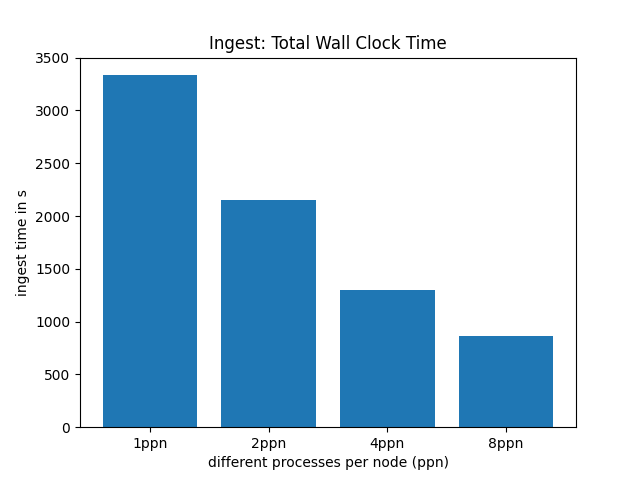
\includegraphics[height=0.9\textwidth]{./analysis/wallclocktime.png}
        \end{figure}
      \end{column}
      \begin{column}{0.5\textwidth}
        \begin{itemize}
          \item Wall clock time decreases when increasing processes per node
          \item More ingestion parallelism increases performance
          \item But sublinear scaling
            \begin{itemize}
              \item Less efficient per extra ingestor process
            \end{itemize}
        \end{itemize}
      \end{column}
    \end{columns}
  \end{frame}
  \begin{frame}{Results}
    \begin{columns}
      \begin{column}{0.5\textwidth}
        \begin{figure}
          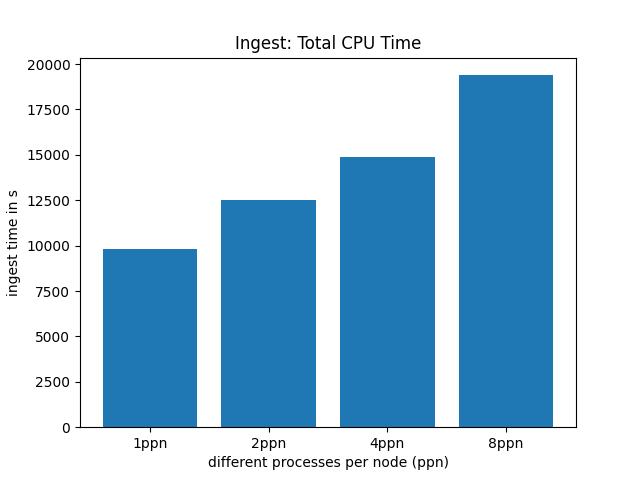
\includegraphics[height=0.9\textwidth]{./analysis/cputime.png}
        \end{figure}
      \end{column}
      \begin{column}{0.5\textwidth}
        \begin{itemize}
          \item CPU time:\\ Wall clock $\cdot$ number of processes
          \item It becomes less CPU efficient with more ingestion nodes
          \item If linear scaling in last plot $\Rightarrow$ the CPU ingestion time would stay the same
        \end{itemize}
      \end{column}
    \end{columns}
  \end{frame}
  \begin{frame}{Results}
    \begin{columns}
      \begin{column}{0.5\textwidth}
        \begin{figure}
          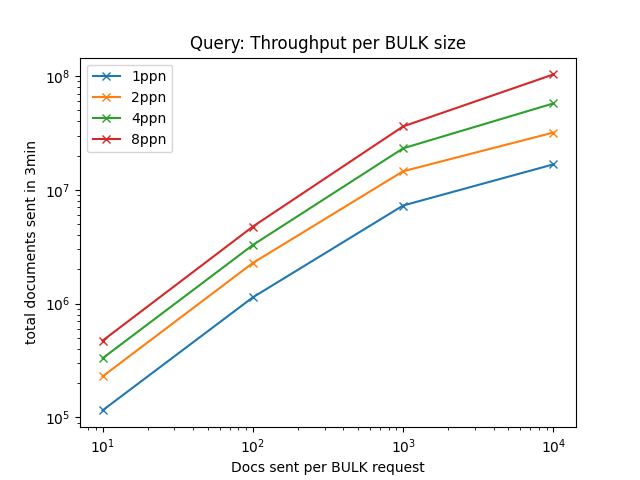
\includegraphics[height=0.9\textwidth]{./analysis/querythroughput.png}
        \end{figure}
      \end{column}
      \begin{column}{0.5\textwidth}
        \begin{itemize}
          \item Works as expected
          \item When sending more documents per request, the HTTP overhead should decrease
          \item This works for all ppn
          \item Increase becomes sublinear
        \end{itemize}
      \end{column}
    \end{columns}
  \end{frame}
  \begin{frame}{Results}
    \begin{columns}
      \begin{column}{0.5\textwidth}
        \begin{figure}
          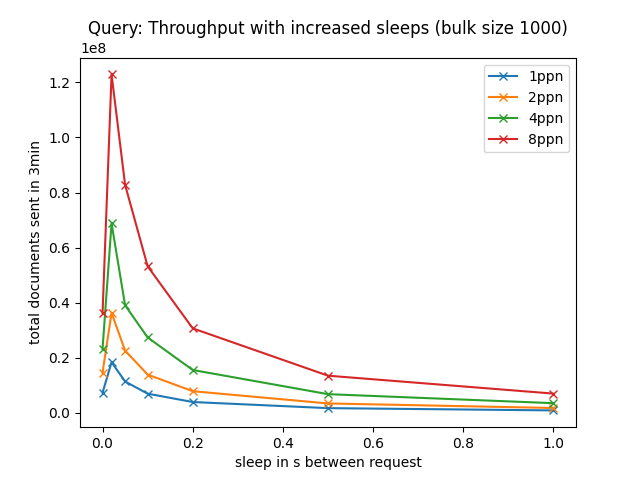
\includegraphics[height=0.9\textwidth]{./analysis/querythroughputsleep.png}
        \end{figure}
      \end{column}
      \begin{column}{0.5\textwidth}
        \begin{itemize}
          \item Sleeping 0.02s is more efficient than not sleeping between requests!
          \item 0.2s is approximately as efficient as 0.0s.
          \item After that, it becomes less efficient since the Elasticsearch is idling.
          \item Possible explaination: Additive Increase, Multiplicative Decrease (AIMD) in TCP, see report
        \end{itemize}
      \end{column}
    \end{columns}
  \end{frame}

	\section{Conclusion}
  \begin{frame}{Challenges/Open Problems}
    \begin{itemize}
      \item Limited response size, hard limit by Elasticsearch's architecture
      \item Not possible to map load generator to cluster node according to optimal network topology
      \item Load generators and clusters cant share the same node
      \item Elasticsearch requires a custom kernel setting
    \end{itemize}
  \end{frame}

	\begin{frame}{Summary}
		\label{pg:lastpage} % Label on last frame to get the page number for footer
    \begin{itemize}
      \item Project was a success, fully implemented both workflow and benchmarker
      \item Zero configuration needed once the benchmark was initially designed
      \item Fully integrated into SLURM
      \item Contributions:
        \begin{enumerate}
          \item On-demand Elasticsearch Cluster Spawner
          \item Ingestion Benchmarker
          \item Query Benchmarker
          \item Example workflow for canonical dataset
        \end{enumerate}
    \end{itemize}
	\end{frame}
\begin{frame}[allowframebreaks]{References}
\renewcommand*{\bibfont}{\normalfont\scriptsize}
  \printbibliography
\end{frame}

\end{document}
